\documentclass{article}

\usepackage{fontspec}
\usepackage{graphicx}
\usepackage{geometry}
\usepackage{listings}
\usepackage[dvipsnames, svgnames, x11names]{xcolor}
\usepackage{fontspec}
\usepackage{mathtools}
\usepackage{verbatim} 
\usepackage{amsthm}
\usepackage{fancyhdr}
\usepackage{minted}
\usepackage{verbatim}
\usepackage{pdfpages}
\usepackage{setspace}
\usepackage{multirow}
\usepackage{multicol}
\usepackage{booktabs}
\usepackage{enumitem}
\usepackage{indentfirst}
\usepackage[colorlinks=true]{hyperref}
\usepackage[BoldFont,SlantFont,CJKchecksingle]{xeCJK}
\usepackage[utf8x]{inputenc}

\linespread{1.5}
\geometry{left=2cm,right=2cm,top=3cm,bottom=3cm}

\usemintedstyle{colorful}
\setminted[c++]{linenos, framesep=2mm, baselinestretch=1.0, breaklines, mathescape, bgcolor=LavenderBlush1}
\setminted[c]{linenos, framesep=2mm, baselinestretch=1.0, breaklines, mathescape, bgcolor=LavenderBlush1}
\setminted[rust]{linenos, framesep=2mm, baselinestretch=1.0, breaklines, mathescape, bgcolor=LavenderBlush1}
\setminted[batch]{linenos, framesep=2mm, baselinestretch=1.0, breaklines, mathescape, bgcolor=LavenderBlush1}
\setminted[bash]{linenos, framesep=2mm, baselinestretch=1.0, breaklines, mathescape, bgcolor=LavenderBlush1}
\setminted[shell]{linenos, framesep=2mm, baselinestretch=1.0, breaklines, mathescape, bgcolor=LavenderBlush1}
\setminted[text]{linenos, framesep=2mm, baselinestretch=1.0, breaklines, mathescape, bgcolor=LavenderBlush1}

\title{SwornDisk Linux Rust Documentation}
\date{\today}

\begin{document}
  \begin{titlepage}
  \maketitle
  \end{titlepage}

  \tableofcontents
  \clearpage

  \section{代码组织}

\subsection{代码目录结构}

\href{https://github.com/occlum/sworndisk-linux-rs}{sworndisk-linux-rs} 仓库包含 \href{https://github.com/Rust-for-Linux/linux}{rust-for-linux} 的完整代码和 \href{https://github.com/occlum/sworndisk-linux-rs/tree/rust/modules/sworndisk}{SwornDisk 内核模块}代码,后者位于 modules/sworndisk 目录下:

\begin{minted}{shell}
  |- .cargo
  |   |- config.toml     # 项目 Cargo 配置文件,主要指定了使用 rustc 时需要附加的编译参数
  |- deps                # 项目依赖的 crates 目录
  |   |- cmwq            # Linux 工作队列 (CMWQ) 封装
  |   |- crypto          # Linux 内核加密 API 封装
  |   |- device-mapper   # Linux 块 I/O  (bio) 与 Device Mapper 框架封装
  |- dm-sworndisk        # SwornDisk Device Mapper 内核模块源码目录
  |   |- Cargo.toml
  |   |- src
  |       |- constant.rs      # 定义 SwornDisk 常量,如块、段大小等
  |       |- context.rs       # 定义用于储存 SwornDisk 上下文的结构,如各个段的实例
  |       |- handler.rs       # 定义处理 Device Mapper 事件 (ctr, dtr, map) 的方法
  |       |- lib.rs           # SwornDisk 内核模块入口 (entry)
  |       |- prelude.rs
  |       |- regions              # 磁盘布局区域实现
  |       |   |- checkpoint       # Checkpoint 区域
  |       |   |   |- bitc.rs      # BIT Category
  |       |   |   |- dst.rs       # Data Segment Table
  |       |   |   |- mod.rs     
  |       |   |   |- svt.rs       # Segment Validity Table
  |       |   |- data             # 数据段区域
  |       |   |   |- mod.rs
  |       |   |   |- segment.rs
  |       |   |- index            # 索引段区域
  |       |   |   |- bit.rs       # Block Index Table (BIT) 实现
  |       |   |   |- memtable.rs  # MemTable 实现
  |       |   |   |- mod.rs
  |       |   |   |- record.rs    # Record 结构
  |       |   |   |- segment.rs   # 索引段结构实现
  |       |   |- mod.rs
  |       |   |- superblock.rs    # 超级块
  |       |- types.rs         # 类型定义
  |       |- unittest.rs      # 单元测试
  |       |- utils            # 数据结构和工具函数
  |       |   |- bitmap.rs          # BitMap
  |       |   |- debug_ignore.rs    # debug_ignore crate 实现
  |       |   |- linked_list.rs     # Rust LinkedList 实现
  |       |   |- lru.rs             # LRU 缓存实现
  |       |   |- mod.rs
  |       |   |- traits.rs          # 需要的 traits 定义 (Serialize, Deserialze..)
  |       |- workers
  |           |- compaction.rs      # Major Compaction 逻辑
  |           |- io.rs              # 处理 I/O 请求
  |           |- mod.rs
  |-- Kbuild
  |-- Makefile
  |-- README.md
  |-- scripts
      |-- fio.conf            # fio 性能测试配置文件
      |-- generate_cmd.sh     # 生成编译时所需的 cmd 文件
      |-- insmod.sh           # 加载内核模块、创建 SwornDisk 示例命令
      |-- restore.sh          # 卸载内核模块、卸载 SwornDisk 示例命令
\end{minted}

\subsection{rust-for-linux}

\subsubsection{原理}

\begin{figure}[H]
  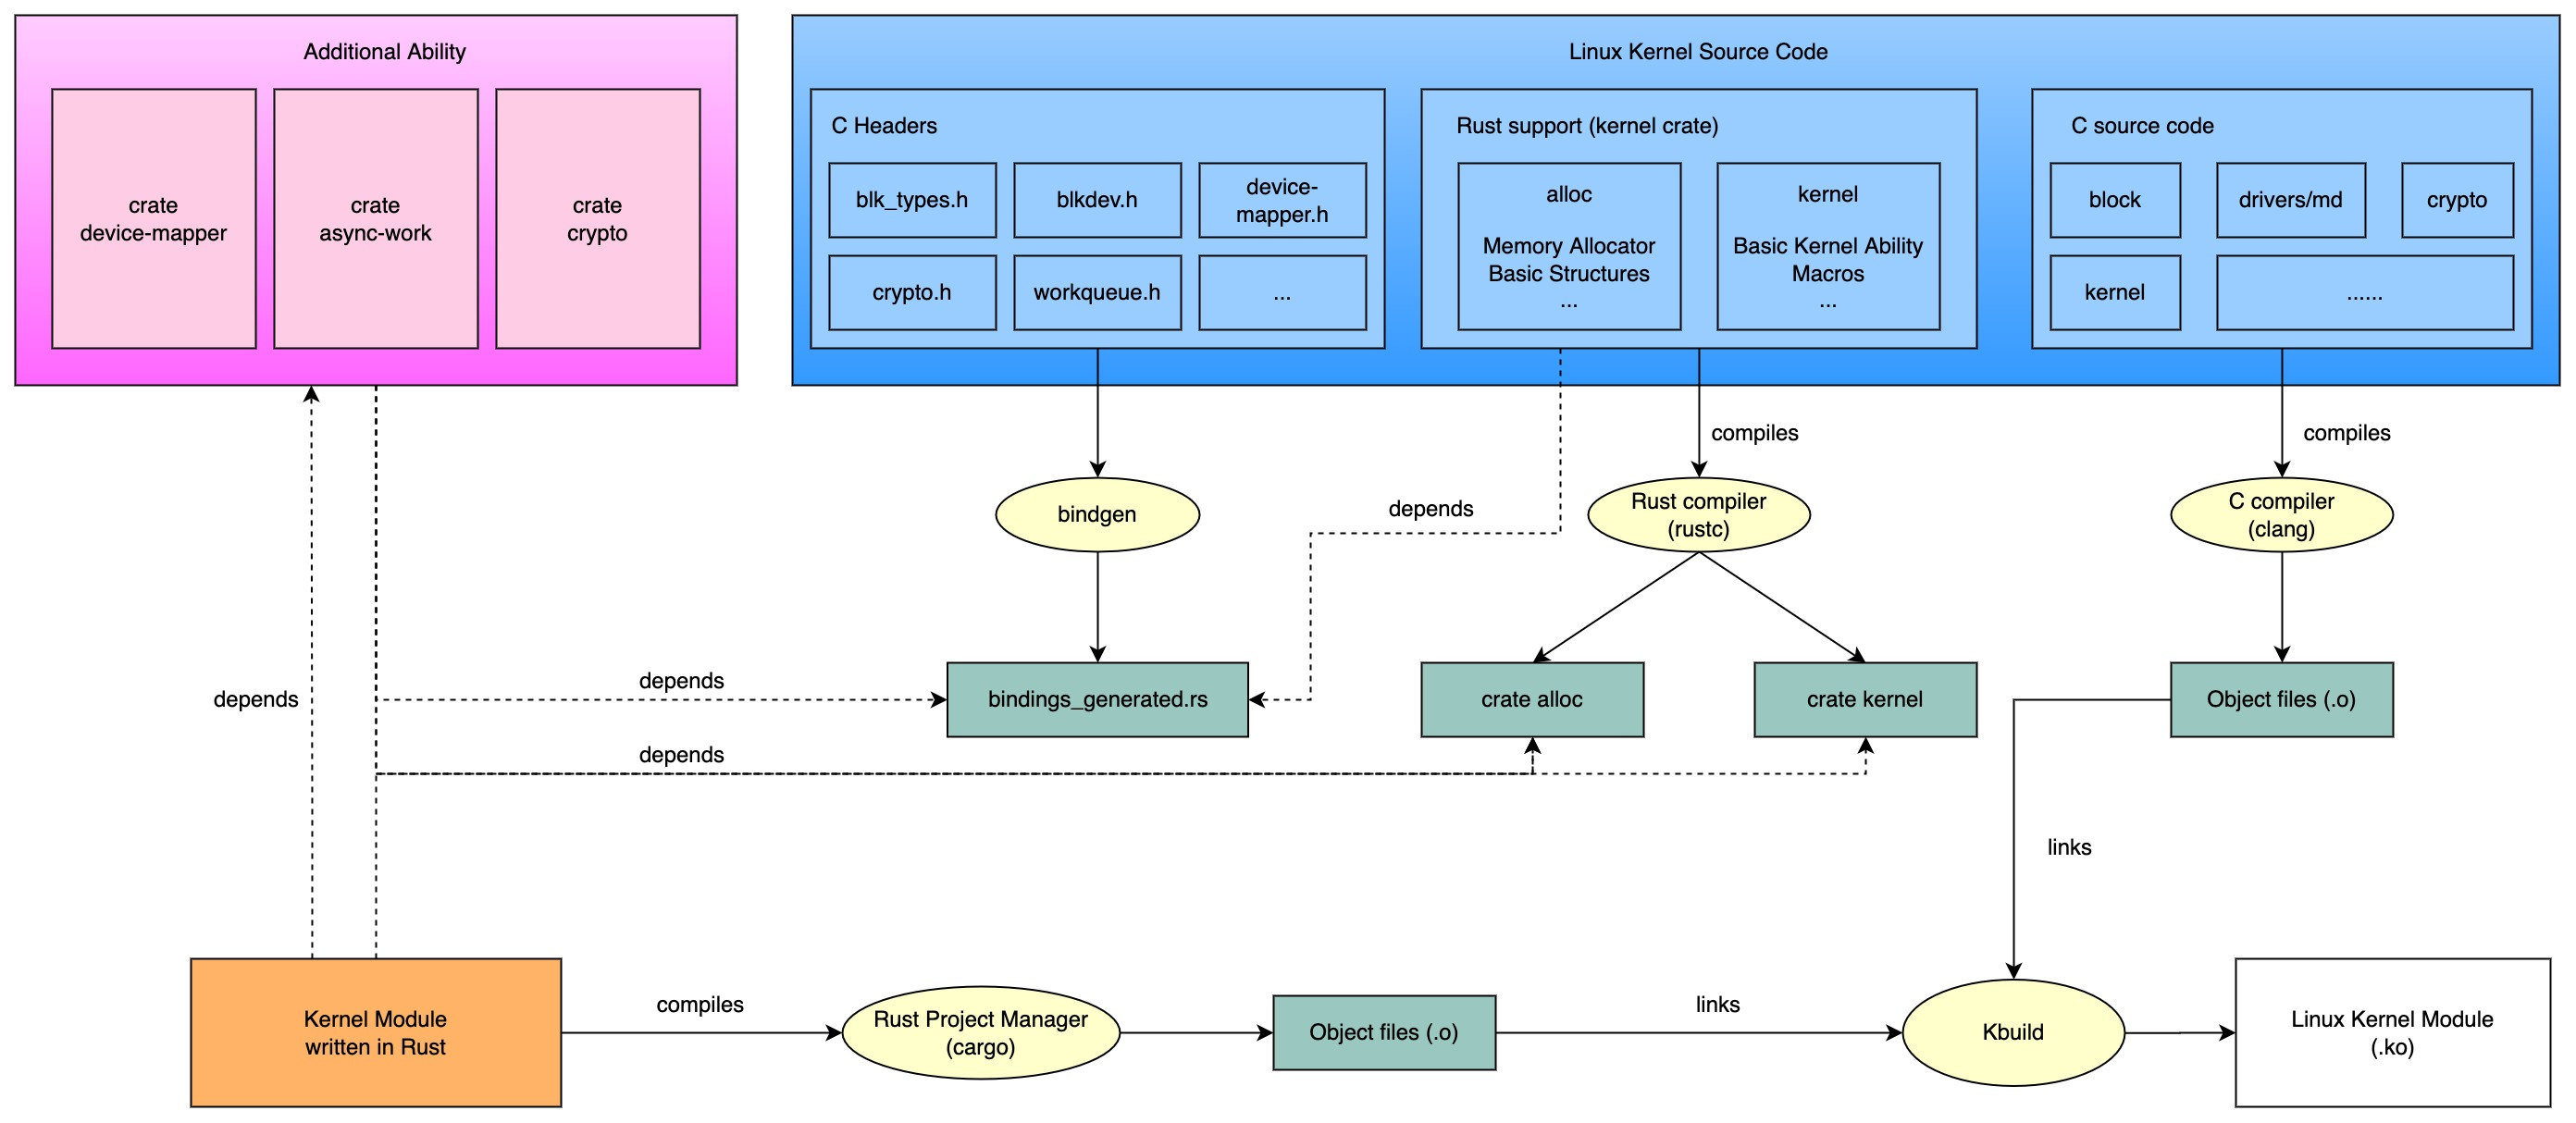
\includegraphics[width=\textwidth]{images/rust-for-linux-ability.jpg}
  \caption{基于 rust-for-linux 编写内核模块的原理图}
  \label{rust-for-linux-kernel-module-theory}
\end{figure}

图 \ref{rust-for-linux-kernel-module-theory} 展示了:

\begin{itemize}
  \item \textbf{rust-for-linux 项目提供 Rust 支持的方式}
  \begin{itemize}
    \item 首先,该项目提供了一套工具链 (rustc, bindgen, ...),并在内核的 Makefile 中定义了如何编译、链接与处理 Rust 源代码。
    \item 在内核的源码树中加入了 Rust 语言的核心能力 (alloc, core),并通过一个 \mintinline{text}{helper.h} 引入需要的 Linux 内核头文件,利用 bindgen 生成 \mintinline{text}{bindings_generated.rs} 文件。
    \item \mintinline{text}{bindings_generated.rs} 文件包含与上述头文件定义的 C 函数签名对应的 Rust 函数(除宏定义和 inline 函数,如果要在 Rust 中使用宏或 inline 函数则需要通过重新定义一个代理 \mintinline{text}{rust_helper_...} 来实现)。
    \item 根据 bindings 封装了一套使用 Linux 部分内核能力的 crate:\mintinline{text}{kernel},封装了如红黑树、互斥锁等 Linux 内核功能。
  \end{itemize}

  \item \textbf{向 rust-for-linux 拓展功能的方式}
  \begin{itemize}
    \item 第一种方法是直接向 \mintinline{text}{kernel} crate 添加内容。在 out-of-tree 的内核模块中,可以直接使用 kernel crate 中的内容。
    \item 第二种方法是将需要添加的内容独立成一个 crate,通过 Rust 的 extern crate 声明对 alloc, core, kernel 的依赖,然后在使用 rustc 编译时添加链接参数 \mintinline{text}{-L/path/to/xxx.o} 链接 alloc, core, kernel 等 crate.
  \end{itemize}

  \item \textbf{使用 Rust 编写内核模块的流程} \quad 根据 rust-for-linux 的 Makefile 中提供的对 .rs 文件的处理方式,分别经过 rustc 编译、ld.lld 链接,经过 modpost, lto 等一系列操作产生 .ko 格式的内核模块。
\end{itemize}

\subsubsection{在 rust-for-linux 上做出的改动}

尽管 SwornDisk 对 rust-for-linux 项目添加的能力 (Device Mapper 等) 都通过独立于内核代码的 crate 形式实现,但由于 rust-for-linux 本身在 API 设计上有一些问题无法满足我们的需求,因此对 rust-for-linux 项目本身也有少量的修改,包括:

\begin{itemize}
  \item 在 \mintinline{text}{rust/kernel/bindings_helper.h} 中添加了所需要的内核 C API 所在的头文件引用。
  \item 在 \mintinline{text}{rust/kernel/lib.rs} 中,修改了 \mintinline{rust}{ThisModule} 的成员可见性为 \mintinline{rust}{pub}。
  \item 在 \mintinline{text}{rust/helpers.c} 中添加了一些 inline 函数或宏的 binding 函数,以 \mintinline{c}{rust_helper_<function_name>} 的形式给出。
  \item 修改了 \mintinline{text}{Makefile} 和 \mintinline{text}{scripts/Makefile.build} 中与 Rust 编译相关的部分,主要是添加或去除了某些参数。
\end{itemize}


\subsubsection{基于 rust-for-linux 添加的内容}

为了实现 SwornDisk,我们主要补充了关于块 I/O, Device Mapper, 内核加密 API 和内核工作队列 CMWQ 的支持。

\begin{table}[H]
  \caption{Rust 容器与 C 结构体对应关系表}
  \begin{center}
  \begin{tabular}{ccc}
  \toprule
  C 结构                              & 对应 Rust 容器                  & 作用              \\
  \midrule
  \textit{struct block\_device}       & \textit{device\_mapper::BlockDevice}   & 表示块设备信息       \\ 
  \textit{struct bio}                 & \textit{device\_mapper::Bio}           &  表示块 I/O 请求信息 \\ 
  \textit{struct target\_type}        & \textit{device\_mapper::TargetType}  & 表示 Device Mapper 目标设备类型信息         \\ 
  \textit{struct dm\_dev}             & \textit{device\_mapper::DmDev}       & 表示 Device Mapper 映射的虚拟设备         \\ 
  \textit{struct dm\_target}          & \textit{device\_mapper::DmTarget}    & 表示 Device Mapper 目标设备实例         \\ 
  \textit{struct dm\_block\_manager}  & \textit{device\_mapperDmBlockManager}       & \multirow{2}{*}{用于 Device Mapper 中块设备的读写} \\ 
  \textit{struct dm\_block}           & \textit{device\_mapperDmBlock}              &                                       \\ 
  \textit{struct dm\_io\_region}      & \textit{device\_mapper::DmIoClient}       &                                       \\ 
  \textit{struct dm\_io\_request}     & \textit{device\_mapper::DmIoRequest}      &                                       \\ 
  \hline
  \textit{struct crypto\_aead}        & \textit{crypto::Aead}         & AEAD 加密实例 \\ 
  \textit{struct aead\_request}       & \textit{crypto::AeadRequest}  & AEAD 加密请求 \\ 
  \textit{struct scatterlist}         & \textit{crypto::ScatterList}  & Linux 散列表 \\ 
  \hline
  \textit{struct workqueue\_struct}   & \textit{cmwq::WorkQueue}   & CMWQ 工作队列 \\ 
  \textit{struct work\_struct}        & \textit{cmwq::WorkStruct}  & CMWQ 工作结构体 \\ 
  
  
  \bottomrule
  \end{tabular}
  \end{center}
\end{table}

  \clearpage
\section{编译、运行、测试}

\subsection{编译 rust-for-linux}

参考 \href{https://github.com/Rust-for-Linux/linux/blob/rust/Documentation/rust/quick-start.rst}{rust-for-linux Quick Start 文档},编译具有 Rust 支持的内核。

根据使用的发行版不同,编译的方法也可能不同。以 Arch Linux 为例,首先需要安装依赖:

\begin{minted}{bash}
$ sudo pacman -S base-devel clang lld python3 llvm bc cpio
\end{minted}

安装 rustup 工具链:

\begin{minted}{bash}
$ curl --proto '=https' --tlsv1.2 -sSf https://sh.rustup.rs | sh
\end{minted}

克隆 rust-for-linux:

\begin{minted}{bash}
$ git clone git@github.com:occlum/sworndisk-linux-rs.git linux
$ cd linux
\end{minted}

根据 rust-for-linux 的要求设置 Rust 环境,安装必要的组件:

\begin{minted}{bash}
$ rustup override set $(scripts/min-tool-version.sh rustc)
$ rustup component add rust-src
$ cargo install --locked --version $(scripts/min-tool-version.sh bindgen) bindgen

$ rustup component add rustfmt
$ rustup component add clippy
\end{minted}

\textbf{PS: 由于 rust-for-linux 项目强制使用 nightly 版本的工具链,SwornDisk 使用的 Rust 版本为 rustc 1.60.0-nightly (9ad5d82f8 2022-01-18),在安装 Rust 工具链时,请务必手动切换到此版本:}

\begin{minted}{bash}
$ rustup toolchain install nightly-2022-01-18
\end{minted}

导出当前系统的内核配置:

\begin{minted}{bash}
$ zcat /proc/config.gz > .config
\end{minted}

编辑 \mintinline{text}{.config} 启用以下选项:

\begin{minted}{text}
CONFIG_RUST_IS_AVAILABLE=y 
CONFIG_RUST=y 
CONFIG_DM_PERSISTENT_DATA=y 
CONFIG_DM_BUFIO=y 
CONFIG_LIBCRC32C=y 
CONFIG_BLK_DEV_LOOP=y 
CONFIG_BLK_DEV_DM=y 
CONFIG_BLK_DEV_LOOP_MIN_COUNT=8
\end{minted}

\textbf{PS: 部分选项可能由于依赖或其它各种原因,在 \mintinline{text}{.config} 中无法配置,此时可以修改 \mintinline{text}{include/config/auto.conf} 文件。}

编译内核:

\begin{minted}{bash}
$ make LLVM=1 -j8
$ sudo make modules_install
\end{minted}

参考 \href{https://wiki.archlinux.org/title/Kernel_(%E7%AE%80%E4%BD%93%E4%B8%AD%E6%96%87)/Traditional_compilation_(%E7%AE%80%E4%BD%93%E4%B8%AD%E6%96%87)}{Kernel - ArchWiki} 更新 initcpio 和 grub,重启即可。

附:\href{https://kirainmoe.feishu.cn/wiki/wikcnyStut2uUsg0RBWGwtOoaPc}{Ubuntu 下编译 rust-for-linux 的过程记录}供参考。

\subsection{编译 SwornDisk}

SwornDisk Rust 源码位于 \mintinline{text}{modules/sworndisk} 中。

\begin{minted}{bash}
$ cd modules/sworndisk
$ make clean
$ make
\end{minted}

若一切正常,应当得到 SwornDisk Linux 内核模块 \mintinline{text}{dm-sworndisk.ko}:

\begin{minted}{bash}
$ modinfo dm-sworndisk.ko

filename:       /home/bellaris/Workspace/linux/modules/sworndisk/dm-sworndisk.ko
author:         Occlum Team
description:    Rust implementation of SwornDisk based on Linux device mapper.
license:        GPL v2
vermagic:       5.17.0-rc8-126275-g6b600e79f6e6-dirty SMP preempt mod_unload 
name:           dm_sworndisk
retpoline:      Y
depends:        
srcversion:     4BAC5027D1352F0DF2B3A7E
parm:           run_unittest:Run dm-sworndisk kernel module unit test (bool)
\end{minted}

\subsection{加载并创建 SwornDisk}

首先加载 SwornDisk 内核模块:

\begin{minted}{bash}
$ sudo insmod dm-sworndisk.ko
\end{minted}

SwornDisk Linux Rust 需要挂载两个物理设备分区(数据设备、元信息设备),我们用 \mintinline{text}{dd} 创建空磁盘文件,使用 \mintinline{text}{losetup} 挂载为回环设备:

\begin{minted}{bash}
$ dd if=/dev/null of=~/tmp/disk.img seek=58593750   # 30GB Data
$ dd if=/dev/null of=~/tmp/meta.img seek=8388608    # 4GB Meta
$ sudo losetup /dev/loop0 ~/tmp/disk.img
$ sudo losetup /dev/loop1 ~/tmp/meta.img
\end{minted}

使用 \mintinline{text}{dmsetup} 创建 SwornDisk Device Mapper 目标设备:

\begin{minted}{bash}
$ echo -e '0 58593750 sworndisk /dev/loop0 /dev/loop1 0 force' | sudo dmsetup create test-sworndisk
\end{minted}

命令用法:

\begin{minted}{bash}
echo -e '0 <size> sworndisk <data_dev> <meta_dev> 0 force' | sudo dmsetup create <name>
\end{minted}

\begin{itemize}[itemsep=2pt,topsep=0pt,parsep=0pt]
  \item \mintinline{text}{<size>}: 磁盘扇区数量,扇区大小为 512B
  \item \mintinline{text}{<data_dev>}: 数据磁盘对应设备文件
  \item \mintinline{text}{<meta_dev>}: 元数据磁盘对应设备文件
  \item \mintinline{text}{<format>}: 是否格式化创建磁盘:(force: 强制格式化创建新磁盘, true: 损坏时格式化, false: 不格式化)
  \item \mintinline{text}{<name>}: 磁盘名称
\end{itemize}

此时成功创建了一个名为 \mintinline{text}{test-sworndisk} 的虚拟块设备,位于 \mintinline{text}{/dev/mapper/test-sworndisk}.

\subsection{测试}

\subsubsection{fio 性能测试}

\mintinline{text}{scripts/fio.conf} 中定义了 fio 测试的配置。

\begin{minted}{bash}
$ sudo fio scripts/fio.conf
\end{minted}

\subsubsection{单元测试}

由于使用 Rust 编写的 Linux 内核模块无法直接使用 \mintinline{text}{cargo test} 进行单元测试,因此单独写了一个模块 \mintinline{text}{unitest} 实现单元测试。在加载内核模块时带参数 \mintinline{text}{run_unittest=true} 即可。

\begin{minted}{bash}
$ sudo insmod dm-sworndisk.ko run_unittest=true
\end{minted}
  \clearpage
\section{核心逻辑}

\subsection{初始化 SwornDisk Device Mapper 目标设备}

\mintinline{text}{DmSwornDiskHandler::ctr (dm-sworndisk/src/handler.rs:28)}

初始化并创建 SwornDisk 虚拟块设备通过 \mintinline{text}{dmsetup} 命令完成,执行该命令时会触发 SwornDisk 的 \mintinline{c}{dm_ctr_fn} (constructor) 回调函数。在 ctr 函数中,主要做的事情是向系统注册 SwornDisk 虚拟块设备、读取或创建 SwornDisk 的关键数据结构,初始化 SwornDisk 的上下文对象。具体地来说:

\begin{itemize}[itemsep=2pt,topsep=0pt,parsep=0pt]
  \item 解析 dmsetup 的参数,获取数据磁盘和元数据磁盘的设备路径
  \item 在 Device Mapper 的 table 中注册设备
  \item 从 meta device 中读取或初始化超级块、Checkpoint
  \item 创建数据段缓冲区、索引段实例、MemTable、工作队列和 bio 处理队列等
  \item 创建 BIT 缓存
  \item 将所有在 SwornDisk 生命周期所需用到的结构与对象包装到 SwornDiskContext 中
\end{itemize}

\subsection{卸载 SwornDisk Device Mapper 目标设备}

\mintinline{text}{DmSwornDiskHandler::dtr (dm-sworndisk/src/handler.rs:175)}

从系统的 Device Mapper table 中释放 SwornDisk 注册的虚拟块设备。

\subsection{处理 bio}

\mintinline{text}{DmSwornDiskHandler::map (dm-sworndisk/src/handler.rs:191)}

SwornDisk Linux Rust 目前实现了三种磁盘 I/O 请求的处理:\textbf{读 (READ)、写 (WRITE)、刷盘 (FLUSH)}. 

\begin{itemize}[itemsep=2pt,topsep=0pt,parsep=0pt]
  \item 当有上述三种类型的 bio 请求到达时,将会首先调用 SwornDisk 的 \mintinline{text}{dm_map_fn} 函数进行处理,将其加到 \mintinline{rust}{SwornDiskContext} 中的 bio 队列 \mintinline{rust}{ctx.bio_queue}  中。这是一个全局共享的 bio 队列,因此对其进行读取或修改前需要先加锁。
  \item 将处理 I/O 的 worker \mintinline{rust}{crate::workers::IoWorker} 加入全局 CMWQ 中(同一个 worker 只会被加入到工作队列一次)。
  \item 返回 \mintinline{rust}{DM_MAPIO_SUBMITTED} 状态码或 \mintinline{rust}{DM_MAPIO_KILL} 状态码(如果 bio 的类型未被支持)。
\end{itemize}

将 bio 加入队列之后,后续对 bio 的处理逻辑均在 \mintinline{rust}{IoWorker} 中完成:\mintinline{text}{dm-sworndisk/src/workers/io.rs:12}.

\subsection{写入数据}

\mintinline{text}{IoWorker::handle_write_request (dm-sworndisk/src/workers/io.rs:160)}

处理写入请求的步骤:

\begin{itemize}[itemsep=2pt,topsep=0pt,parsep=0pt]
  \item 首先计算 bio 请求的扇区号所对应的 LBA 范围;
  \item 根据 LBA 将 bio 的数据拆成若干个块大小的分片;
  \item 对于每个 LBA 及其对应的数据分片,将数据以明文形式写入 SwornDiskContext 中的数据段缓冲区中 \mintinline{rust}{ctx.data_seg_buffer},并维护 LBA 与数据的对应关系。
  \item 写入时会首先更新 Checkpoint 中的 DST,分配一个新的可用块。如果当前 LBA 的记录已存在,执行原地更新。
  \begin{itemize}[itemsep=2pt,topsep=0pt,parsep=0pt]
    \item 如果此时数据段缓冲区已写满,则触发\textbf{将数据段缓冲区写回磁盘数据段}的操作:
    \item 对于数据段中所有 LBA 及对应的明文数据,随机生成 key, nonce 使用 AES-128-GCM 算法进行加密,并得到 MAC
    \item 将 \mintinline{text}{LBA → (HBA, key, nonce, MAC)} 的对应关系记录 (Record) 写入 MemTable 中
    \item 清空数据段缓冲区,并从 Checkpoiint 的 DST 中请求分配一个新的数据段。
  \end{itemize}
  \item 如果 MemTable 写满(Record 数量达到阈值),将触发 minor compaction
  \begin{itemize}[itemsep=2pt,topsep=0pt,parsep=0pt]
    \item 使用 MemTable 中的 Record 创建 BIT
    \item 将 BIT 根节点的信息写入 Checkpoint 的 BITCagetory 中
    \item 清空当前 MemTable
    \item 检查当前是否需要进行 major compaction, 如果需要则创建一个 compaction worker 加入工作队列中
  \end{itemize}
  \item 调用 \mintinline{rust}{bio.end()} 结束 bio 请求
\end{itemize}

\subsection{读取数据}

\mintinline{text}{IoWorker::handle_read_request (dm-sworndisk/src/workers/io.rs:60)}

处理读取请求的步骤:

\begin{itemize}[itemsep=2pt,topsep=0pt,parsep=0pt]
  \item 首先计算 bio 请求的扇区号所对应的 LBA 范围;
  \item 对于每个 LBA:
  \begin{itemize}[itemsep=2pt,topsep=0pt,parsep=0pt]
    \item 首先从数据段缓冲区中,查找是否有对应该 LBA 的明文数据,若有则直接填入 bio
    \item 接下来从 MemTable 中,查找是否有对应该 LBA 的加密信息 Record,若有则根据 Record 中的 HBA, Key, nonce 和 MAC 从磁盘数据段读入对应的块并解密,返回给 Bio
    \item 如果请求的 LBA 不在 MemTable 中,接下来按照层级有小到大、最后修改时间的逆序遍历 dsLSM-tree 中的 BIT,查找对应该 LBA 的加密信息(查找 LBA 时需要先通过 BIT 节点记录的 \mintinline{rust}{lba_range} 判断当前 LBA 是否在此 BIT 节点中,在单个 BIT 节点中查找的复杂度为 $O(\log n)$),若找到 Record 则根据其中的 HBA, Key, nonce 和 MAC 从磁盘数据段读入对应的块并解密,并返回给 bio
    \item 在从 BIT 索引的过程中,会将读到的 BIT 中间节点或叶节点,缓存到 SwornDiskContext 的 BIT 节点块缓存 (\mintinline{text}{ctx.indirect_block_cache, ctx.leaf_block_cache}) 中。
  \end{itemize}
  \item 调用 \mintinline{rust}{bio.end()} 结束 bio 请求
\end{itemize}

\subsection{BlockIndexTable (BIT) 实现}

SwornDisk Linux Rust 对 BIT 的实现是\textbf{直接在磁盘上以块为单位维护 BIT},如图\ref{swrodnsik-rust-bit}所示:

\begin{figure}[H]
  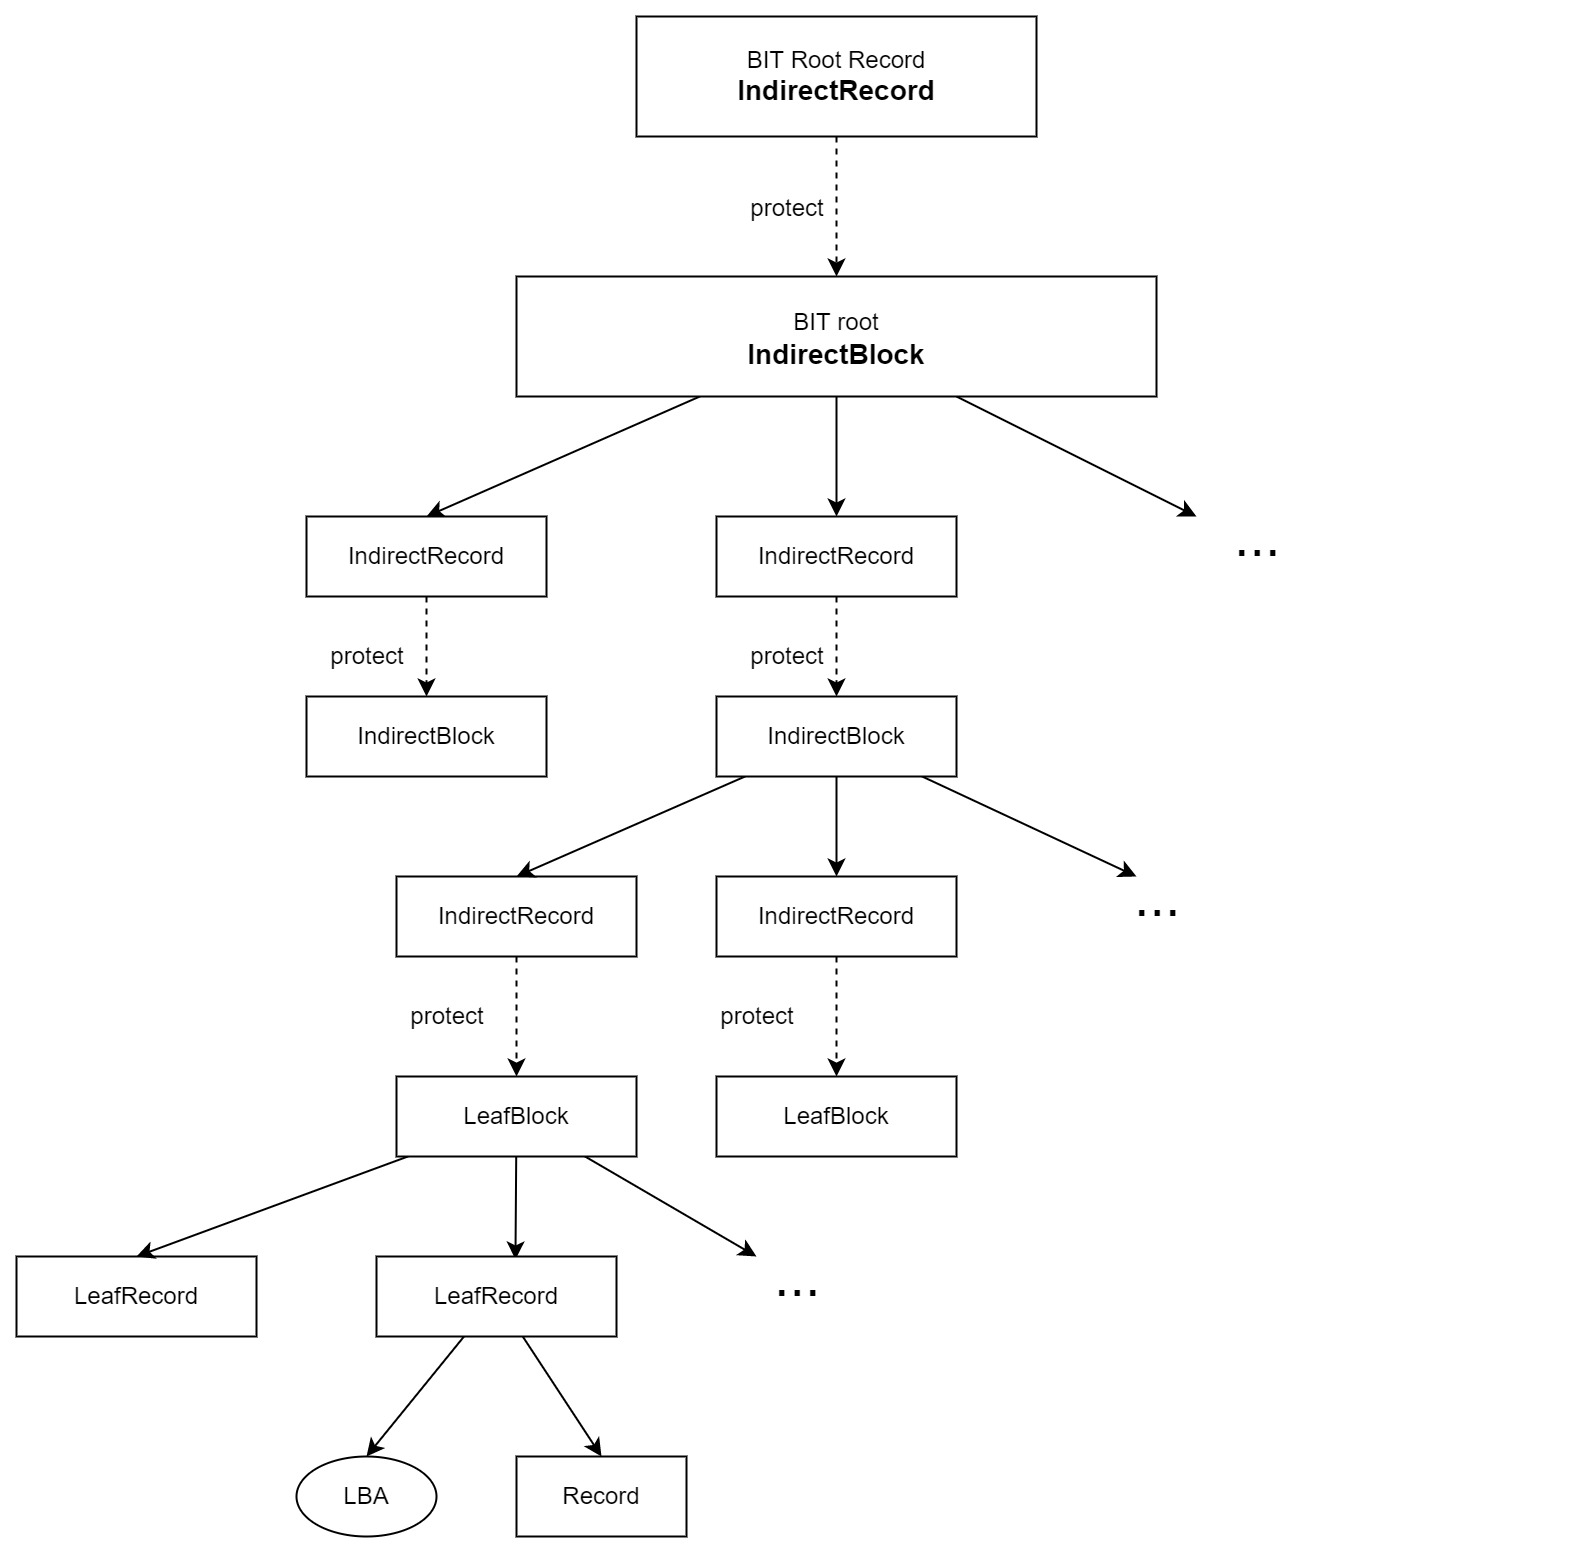
\includegraphics[width=0.8\textwidth]{images/bit-structure.jpg}
  \caption{SwornDisk Linux Rust BIT 结构}
  \label{sworndisk-rust-bit}
\end{figure}

BIT 的节点以块为单位组织,分为两类:IndirectBlock 和 LeafBlock;每个块都被 IndirectRecord 结构保护,维护了节点块的 HBA, key, MAC, nonce 和节点的 LBA 范围。

\clearpage
\subsubsection{数据结构定义}

\begin{minted}{rust}
/// BIT Record
#[derive(Copy, Clone, Debug)]
pub struct Record {
    /// HBA (Hardware Block Address)
    pub hba: u64,
    /// Crypto key
    pub key: KeyType,
    /// Crypto random string (a.k.a nonce / iv)
    pub nonce: NonceType,
    /// Crypto authentication data (a.k.a MAC / tag)
    pub mac: MacType,
}

#[derive(Copy, Clone, Debug)]
/// Leaf node of BIT
pub struct LeafRecord {
    /// logical block address of current record
    pub lba: u64,
    /// hba & key & nonce & mac
    pub record: Record,
}

#[derive(Debug)]
/// On-disk unit of leaf node
pub struct LeafBlock {
    /// number of LeafRecord
    pub count: usize,
    /// children vector
    pub children: Vec<LeafRecord>,
}

#[derive(Copy, Clone, Debug)]
/// Indirect node of BIT
pub struct IndirectRecord {
    /// lba range of IndirectBlock responding to this IndirectRecord
    pub lba_range: (u64, u64),
    /// hba & key & nonce & mac
    pub record: Record,
}

#[derive(Debug)]
/// On-disk unit of indirect node
pub struct IndirectBlock {
    /// number of IndirectRecord
    pub count: usize,
    /// children vector
    pub children: Vec<IndirectRecord>,
}

#[derive(Debug)]
pub struct BIT {
    /// root node of BIT
    pub root: IndirectBlock,

    /// IndirectRecord of root node
    pub record: IndirectRecord,

    /// max level of BIT
    pub level: usize,

    /// element number of BIT
    pub size: usize,
}
\end{minted}

\subsubsection{从 MemTable 创建 BIT}

\mintinline{text}{BIT::from_memtable (dm-sworndisk/src/regions/index/bit.rs:320)}

\begin{itemize}[itemsep=2pt,topsep=0pt,parsep=0pt]
  \item 计算 MemTable 中元素数量所需的 BIT 层级
  \item 分配 LeafBlock 和 IndirectBlock 的缓冲区
  \item 遍历 MemTable 中的 $(lba, record)$,加入 LeafBlock 中
  \item 如果 LeafBlock 或 IndirectBlock 写满,写入磁盘并将该节点的 Record 信息写到上级 IndirectBlock 中,循环完成写回操作
  \item 返回新的 BIT 信息
\end{itemize}

\subsubsection{BIT Compaction}

\mintinline{text}{BIT::from_compaction (dm-sworndisk/src/regions/index/bit.rs:408)}

\begin{itemize}[itemsep=2pt,topsep=0pt,parsep=0pt]
  \item 选取需要被 compaction 的 BIT
  \item 计算 compaction 后产生的 BIT 最大层级
  \item 分配 LeafBlock 和 IndirectBlock 的缓冲区
  \item 为每个 BIT 创建一个迭代器
  \item 遍历每个迭代器,每次选出最小的一个 $(lba, record)$ 元组,加入新的 BIT 中。如果有多个同样 LBA 的 Record,选择最新的 Record 加入 BIT 中
  \item 如果 LeafBlock 或 IndirectBlock 写满,写入磁盘并将该节点的 Record 信息写到上级 IndirectBlock 中,循环完成写回操作
  \item 返回新的 BIT 信息
  \item 删除并释放已经被 compaction 的 BIT
\end{itemize}

  \clearpage

\section{已知局限}

\subsection{SwornDisk Linux Rust 实现的局限}

SwornDisk Rust 目前实现的功能仍然是不完整的,仍未完成的功能有:

\begin{itemize}[itemsep=2pt,topsep=0pt,parsep=0pt]
  \item 垃圾回收 (segment cleaning)
  \item 日志
  \item Checkpoint 数据加密
  \item multi logging head
  \item thread logging
\end{itemize}

同时,SwornDisk 仍未经过性能调优,目前比较突出的问题和可能的原因是:

\begin{itemize}[itemsep=2pt,topsep=0pt,parsep=0pt]
  \item 顺序读的性能不符合预期(较低),分析问题出现在从磁盘中读取块花费的时间比较长
\end{itemize}

此外可能还存在若干未发现的缺陷。

\subsection{工程方案上的局限}

尽管目前初步验证了使用 Rust 实现 Linux 内核模块的可行性,但仍然具有很多局限性。例如:

\begin{itemize}
  \item 尽管 rust-for-linux 提供了使用 Rust 编写 Linux 内核模块的模式,但由于现阶段只提供了 “使用 rustc 编译 .rs 文件” 这种程度的支持,不支持使用 cargo 组织工程,对编写 SwornDisk 这样较复杂的内核模块(尤其是在我们还需要向 rust-for-linux 补充能力的情况下)很不友好。
  \item 我们在实现 SwornDisk Linux Rust 的时候尝试引入了 cargo 来组织工程,使用 cargo 的 workspace 来管理多个 crate,实现了分别编译多个依赖 crate 并生成一个目标文件的功能。但这并不代表着可以在其中随意引入第三方 crate,主要原因如下:
  \begin{itemize}
    \item 内核模块不能依赖标准库 (std)
    \item rust-for-linux 对 Rust 语言的核心能力支持不完整,如其只提供 alloc, core 和 kernel 三个 crate,同时 alloc crate 提供的数据结构也是不完整的(例如没有 LinkedList)
    \item 在 rust-for-linux 中,如果尝试在堆上分配数据(如创建 Vec, Box),都需要使用类似 \mintinline{rust}{try_new()}, \mintinline{rust}{try_push()} 这样返回 \mintinline{text}{Result<T>} 的 API 来创建、分配空间,而不能直接使用 \mintinline{text}{new()} 等创建。这些限制会阻碍我们直接使用开源的 crate.
  \end{itemize}
  \item 使用 Rust 编写的 Linux 内核模块,目前只能在同样具有 Rust 支持的 Linux 内核上编译、运行
  \begin{itemize}
    \item 我们尝试过在具有 Rust 支持的内核上编译产生 .ko,复制到没有 Rust 支持的内核加载,会由于内核的 version magic 不同,导致无法加载。
    \item 如果我们跳过对内核模块的 version magic 检查,直接加载 .ko,会由于找不到 Rust 的 alloc, core 和 rust-for-linux 提供的 kernel crate 中方法的符号,无法加载(alloc, core, kernel 是被链接到具有 Rust 支持的内核中的)。
    \item 尽管我们手动将 alloc, core, kernel 这些 crate 编译出的 .o 文件合并到内核模块的 .o 中,参与最终内核模块的生成;但仍然在其它机器上会找不到部分 Linux 内核中的函数的符号(系 kernel crate 使用的 binding)。
    \item 综上,我们目前可以认为,在没有 Rust 支持的内核上加载 Rust 编写的内核模块较难以实现,而为了加载模块必须重新编译具有 Rust 支持的内核的成本也很高。
  \end{itemize}
\end{itemize}
  \clearpage
\section{经验体会}

\subsection{如何往 rust-for-linux 里面加东西}

主要包含以下几步:

\begin{itemize}[itemsep=2pt,topsep=0pt,parsep=0pt]
  \item 在 \mintinline{text}{rust/kernel/bindings_helper.h} 引入需要的头文件
  \item make 内核重新生成一下 bindings 文件
  \item 在 \mintinline{text}{rust/kernel} crate 中使用 \mintinline{rust}{bindings::xxx}
  \item 或创建新的 crate ,其中声明 \mintinline{rust}{extern crate kernel} 并使用 \mintinline{rust}{kernel::bindings::xxx}
\end{itemize}

\subsection{使用 Cargo 组织工程}

在 rust-for-linux 中使用 cargo 组织工程,主要需要解决两个问题:

\begin{itemize}[itemsep=2pt,topsep=0pt,parsep=0pt]
  \item 在 cargo 调用 rustc 编译的时候,需要添加一系列参数。这部分参数通过 \mintinline{text}{.cargo/config.toml} 声明;由于需要引用内核代码树中的文件,需要注意路径。
  \item cargo 工程类型需要是 rlib, 同时生成的文件需要是 .o 格式的目标文件 (emit=objs);多个 crate 生成的 .o 文件需要使用 ld.lld 合并成一个 .o 文件。
  \item 需要写一个 shell 脚本,给生成的 .o 文件创建一个 .cmd 格式的声明文件,声明该模块的依赖路径和源码路径等(参考 \mintinline{text}{dm-sworndisk/scripts/generate_cmd.sh})。
  \item 接下来的步骤 (modpost, lto, ...) 交给 Linux Kbuild 完成即可。
\end{itemize}

\subsection{如何在 Rust 的 SwornDisk 中管理全局变量}

在实现 SwornDisk 的时候免不了需要用到一些全局共享的东西,由于 rust-for-linux 的诸多限制,所以我们不能用 \mintinline{text}{lazy_static} 来声明全局变量(主要原因是它依赖了 spin 这个 crate 模拟并发原语)。要在全局范围内访问一些内容,主要有两种解决方案:

\begin{itemize}[itemsep=2pt,topsep=0pt,parsep=0pt]
  \item 将值分配在堆上,指针交给某些具有 private 成员的结构体保存。
  \item 使用 \mintinline{rust}{Box<Option<T>>} 结构 (unsafe).
\end{itemize}

\clearpage
\subsection{一些常见的场景的实现}

\subsubsection{如何加解密一个块}

\begin{minted}{rust}
use crypto::{Aead, get_random_bytes};

let mut aead = Aead::new(c_str!("gcm(aes)"), 0, 0).unwrap();

let key = get_random_bytes(16);         // Vec<u8>
let mut nonce = get_random_bytes(12);   // Vec<u8>
let mut plain = get_random_bytes(4096); // Vec<u8>

// 加密
let (mut cipher, mut mac) = aead.as_ref()
  .encrypt(&key, &mut nonce, &mut plain,)
  .unwrap();

// 解密
let plain = aead.as_ref()
  .decrypt(&key, &mut mac, &mut nonce, &mut cipher)
  .unwrap();
\end{minted}

\subsubsection{如何从硬盘读写一个块}

\begin{minted}{rust}
// 分配一个块
let mut block = Vec::new();
block.try_resize(BLOCK_SIZE as usize, 0u8)?;

// 创建一个 DmIoRegion, 注意大小以扇区为单位
// DmIoRegion::new(block_device, sector, nr_sectors) -> Result<DmIoRegion>
let mut region = DmIoRegion::new(&bdev, record.hba, BLOCK_SECTORS)?;

// 创建 Device Mapper I/O 请求
let mut io_req = DmIoRequest::with_kernel_memory(
    READ as i32,                   // 写入请求时此处为 WRITE
    READ as i32,
    block.as_mut_ptr() as *mut c_void,
    0,
    client,                        // DmIoClient
);

// 提交 IO 请求
io_req.submit(&mut region);
\end{minted}

\subsubsection{如何将一个 struct 储存到硬盘上}

由于 rust-for-linux 中不能用标准库,因此也不能用 \mintinline{rust}{io::Read} 和 \mintinline{rust}{io::Write} 这种 trait,此时如何把一个 Rust struct 持久化地保存到硬盘上就成为一个问题。

我们采用的方案是将块二进制序列化,通过实现 \mintinline{rust}{Serialize} 和 \mintinline{rust}{Deserialze} trait 可以将一个 struct 序列化为二进制串(或从二进制串解析出 struct 本身):

\begin{minted}{rust}
/// Serailize trait: convert a struct into binary bufferr (Vec<u8>)
pub trait Serialize {
    fn serialize(&self) -> Result<Vec<u8>>;
}

/// Deserialize trait: convert a binary buffer (&Vec<u8>) into a struct
pub trait Deserialize {
    fn deserialize(buffer: &[u8]) -> Result<Self>
    where
        Self: Sized;
}
\end{minted}

PS: 其实我曾经想尝试一下引入 serde, 不过看起来很麻烦,当时安排比较紧没有那么多时间可以尝试。

\subsubsection{如何创建一个异步任务 (worker) 并加入队列中}

\begin{minted}{rust}
use cmwq::{WorkFuncTrait, WorkQueue, WorkStruct};

struct Worker;

impl WorkFuncTrait for Worker {
  fn work(_work_struct: *mut bindings::work_struct) -> Result {
    // do something...
    // *mut bindings::work_struct can be used for calling `container_of!()`
  }
}

let mut work_queue = WorkQueue::new(c_str!("queue"), bindings::WQ_UNBOUND | bindings::WQ_MEM_RECLAIM, 0)?;

let mut worker = WorkStruct::new();
worker.init::<Worker>();

work_queue.queue_woork(&mut worker);

\end{minted}
\end{document}